%%%%%%%%%%%%%%%%%%%%%%%%%%%%%%%%%%%%%%%%%%%%%%%%%%%%%%%%%%%%%%%%%%%%%%%%%%
%
%    phase1-GO.tex  (use only for General Observer and Snapshot proposals; use phase1-AR.tex for Archival Research and
%                      Theory proposals use phase1-DD.tex for GO/DD proposals and use phase1-MC.tex for GO/MC rapid response
%                       proposals).
%
%    HUBBLE SPACE TELESCOPE
%    PHASE I OBSERVING PROPOSAL TEMPLATE 
%     FOR CYCLE 25 and beyond
%
%    Version 2.1; November 2018
%
%    Guidelines and assistance
%    =========================
%     Cycle 27 Announcement Web Page:
%
%         https://hst-docs.stsci.edu/ 
%
%    Please contact the STScI Help Desk if you need assistance with any
%    aspect of proposing for and using HST. Either send e-mail to
%    help@stsci.edu, or call 1-800-544-8125; from outside the United
%    States, call [1] 410-338-1082.
%
%
%%%%%%%%%%%%%%%%%%%%%%%%%%%%%%%%%%%%%%%%%%%%%%%%%%%%%%%%%%%%%%%%%%%%%%%%%%%

% The template begins here. Please do not modify the font size from 12 point.

\documentclass[12pt]{article}
\usepackage{phase1}
\usepackage{graphicx}
\usepackage{natbib}
\usepackage{graphicx}
%\usepackage{sidecap}
\DeclareRobustCommand{\ion}[2]{%
\relax\ifmmode
\ifx\testbx\f@series
{\mathbf{#1\,\mathsc{#2}}}\else
{\mathrm{#1\,\mathsc{#2}}}\fi
\else\textup{#1\,{\mdseries\textsc{#2}}}%
\fi}


\def\aj{AJ}%

          % Astronomical Journal

\def\araa{ARA\&A}%

          % Annual Review of Astron and Astrophys

\def\apj{ApJ}%

          % Astrophysical Journal

\def\apjl{ApJ}%

          % Astrophysical Journal, Letters

\def\apjs{ApJS}%

          % Astrophysical Journal, Supplement

\def\ao{Appl.~Opt.}%

          % Applied Optics

\def\apss{Ap\&SS}%

          % Astrophysics and Space Science

\def\aap{A\&A}%

          % Astronomy and Astrophysics

\def\aapr{A\&A~Rev.}%

          % Astronomy and Astrophysics Reviews

\def\aaps{A\&AS}%

          % Astronomy and Astrophysics, Supplement

\def\azh{AZh}%

          % Astronomicheskii Zhurnal

\def\baas{BAAS}%

          % Bulletin of the AAS

\def\jrasc{JRASC}%

          % Journal of the RAS of Canada

\def\memras{MmRAS}%

          % Memoirs of the RAS

\def\mnras{MNRAS}%

          % Monthly Notices of the RAS

\def\pra{Phys.~Rev.~A}%

          % Physical Review A: General Physics

\def\prb{Phys.~Rev.~B}%

          % Physical Review B: Solid State

\def\prc{Phys.~Rev.~C}%

          % Physical Review C

\def\prd{Phys.~Rev.~D}%

          % Physical Review D

\def\pre{Phys.~Rev.~E}%

          % Physical Review E

\def\prl{Phys.~Rev.~Lett.}%

          % Physical Review Letters

\def\pasp{PASP}%

          % Publications of the ASP

\def\pasj{PASJ}%

          % Publications of the ASJ

\def\qjras{QJRAS}%

          % Quarterly Journal of the RAS

\def\skytel{S\&T}%

          % Sky and Telescope

\def\solphys{Sol.~Phys.}%

          % Solar Physics

\def\sovast{Soviet~Ast.}%

          % Soviet Astronomy

\def\ssr{Space~Sci.~Rev.}%

          % Space Science Reviews

\def\zap{ZAp}%

          % Zeitschrift fuer Astrophysik

\def\nat{Nature}%

          % Nature

\def\iaucirc{IAU~Circ.}%

          % IAU Cirulars

\def\aplett{Astrophys.~Lett.}%

          % Astrophysics Letters

\def\apspr{Astrophys.~Space~Phys.~Res.}%

          % Astrophysics Space Physics Research

\def\bain{Bull.~Astron.~Inst.~Netherlands}%

          % Bulletin Astronomical Institute of the Netherlands

\def\fcp{Fund.~Cosmic~Phys.}%

          % Fundamental Cosmic Physics

\def\gca{Geochim.~Cosmochim.~Acta}%

          % Geochimica Cosmochimica Acta

\def\grl{Geophys.~Res.~Lett.}%

          % Geophysics Research Letters

\def\jcp{J.~Chem.~Phys.}%

          % Journal of Chemical Physics

\def\jgr{J.~Geophys.~Res.}%

          % Journal of Geophysics Research

\def\jqsrt{J.~Quant.~Spec.~Radiat.~Transf.}%

          % Journal of Quantitiative Spectroscopy and Radiative Trasfer

\def\memsai{Mem.~Soc.~Astron.~Italiana}%

          % Mem. Societa Astronomica Italiana

\def\nphysa{Nucl.~Phys.~A}%

          % Nuclear Physics A

\def\physrep{Phys.~Rep.}%

          % Physics Reports

\def\physscr{Phys.~Scr}%

          % Physica Scripta

\def\planss{Planet.~Space~Sci.}%

          % Planetary Space Science

\def\procspie{Proc.~SPIE}%

          % Proceedings of the SPIE

\let\astap=\aap

\let\apjlett=\apjl

\let\apjsupp=\apjs

\let\applopt=\ao

%

\uchyph=0

%\bibpunct{(}{)}{;}{a}{}{,}

\begin{document}
\section*{Title, Co-Is, etc.}
\textbf{This information will go into the form, the pdf itself must be anonymous. I'm just collecting it here so we have it all in one place for now.}

\textbf{Title:} A pure-parallel search for faint stuff in star forming regions
(acronym: PPS-FS-SF)

\textbf{Please list Co-I Nae, Institution, email address, so I can copy it in the form:}

\pagebreak
%   1. SCIENTIFIC JUSTIFICATION
%       (See https://hst-docs.stsci.edu/display/HSP/HST+Cycle+27+Preparation+of+the+PDF+Attachment)
%
%
\justification          % Do not delete this command.
% Enter your scientific justification here. 
Stars and planetary systems continue to form in our Milky Way today. Images of
these star forming regions are among the most spectacular images ever taken by
the Hubble Space Telescope (HST) (e.g.\ Fig.~\ref{fig:reiter}. Star forming
regions contain structure over a large range of scales. The clouds themselves
range from a few to hundreds of parsecs across; in each cloud dozens to
thousands of stars form. 
When cloud fragments start to collapse into proto stars, they are still deeply
embedded into a dusty envelope and can be seen only in the sub-mm and IR (class
0 sources). Because angular momentum is conserved, infall does not happen
radially all the way down, but instead an accretion disks takes shape, while
the remaining envelope still hides the inner core from view in all but the
far-IR (class I sources).  These early objects often also drive powerful jets
that propagate through the envelope and pierce the cloud. Once the envelope
depletes, the stars become visible in the optical, but accretion from the disk
continues (class II sources). At the same time, grains in the disks coagulate
into planets. Once the disk depletes due to planet formation, accretion or
evaporation, we end up with a planetary system around a young, active star
(class III sources). For late-type stars, this evolution takes several Myrs,
while massive stars can go through a similar sequence much faster; meaning that
they are typically still surrounded by dense cloud material when they reach the main-sequence.
While the central object can be studied from the spectral energy distribution,
we need high-resolution images such as Fig.~\ref{fig:krist}, \ref{fig:reiter},
or \ref{fig:ONCACS} to understand how disks, jets, and the remaining envelope
look, evolve and how they interact.


\begin{figure}
    \centering
    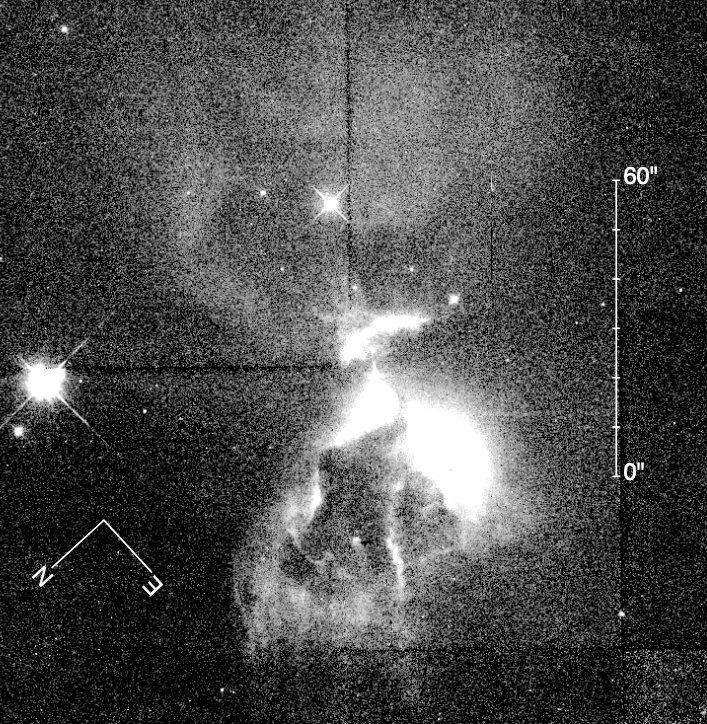
\includegraphics[height=8cm]{Krist98.png}
    \caption{Young, low-mass star FS Tauri in low-mas star forming region observed with WFPC2. The image is combined from several exposures mostly in the F675W filter. Average exposure time is about 800~s. The image reveals a hour-glass shaped reflection nebula and a jet. From: \citet{1998ApJ...501..841K}}
    \label{fig:krist}
\end{figure}




\begin{figure}
    \centering
    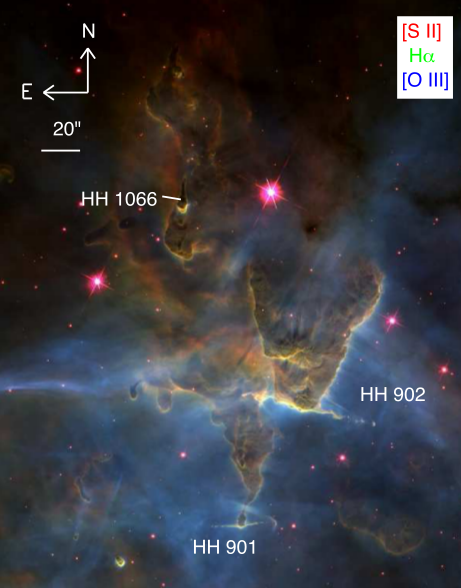
\includegraphics[width=.45\textwidth]{reiter13_fig3.png}
    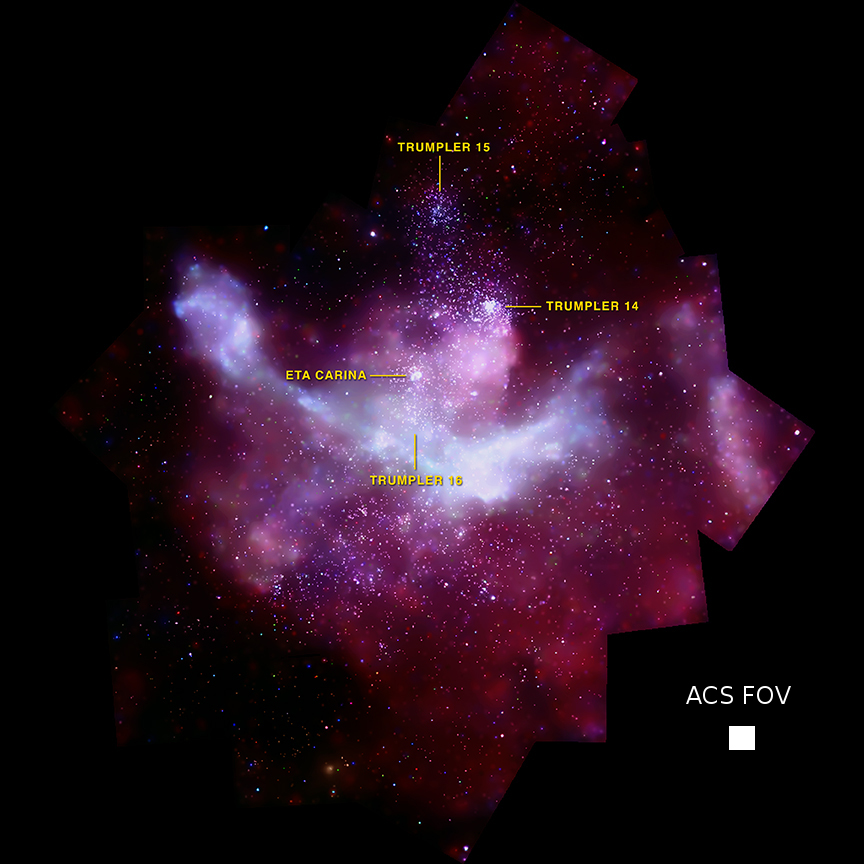
\includegraphics[width=.54\textwidth]{carina_xray_label.jpg}
    \caption{\emph{Left:}Protostellar jets in the Carina region, observed with WFC3 in same filters we propose to use; exposure time about 2000~s for H$\alpha$ and about 3000~s for [O~{\sc iii}]. From: \citet{2013MNRAS.433.2226R} \emph{Right:} X-ray view of the entire Carina star forming region. This image is about 1 degree across and shows that practically any location for a WFC3 or ACS pointing in the star forming region will show young stars with disks (Chandra discovered $> 14,000$ source) and ionized plasma. Image credit: NASA/CXC/PSU/L.Townsley et al.}
    \label{fig:reiter}
\end{figure}

\section{Point sources in the star forming regions}
Chandra has surveyed many of the massive star forming regions in the Milky Way
in X-rays (e.g.\ \citealt{2011ApJS..194....1T} for Carina,
\citealt{2010ApJ...713..871W} for Cyg OB2, \citealt{2005ApJS..160..379F} for
the Orion Nebula Cloud, \citealt{2008AJ....135..693W} for RCW 108) and a
surprising number of the lower-mass star forming regions
(e.g.\ \citealt{2018AJ....155..241W} for Serpens, \citealt{2012AJ....144..101G}
for IRAS 20050+2720, \citealt{2007A&A...468..353G} for the Taurus Molecular
Cloud, using \emph{XMM-Newton} because of its larger field-of-view). Chandra
images reach spatial resolution on sub-arcsecond scales. In the IR, essentially
all star forming regions have been looked at with \emph{Spitzer}
(e.g.\ \citealt{2009ApJS..184...18G} surveyed all star forming regions within 1
kpc, examples for more massive, further regions are XXX). The IR and the hard
X-rays are less extincted than optical wavelength, and thus allow us to view
deeper into the embedded regions. The combination of X-rays and IR information
is a great tool to identify the point soures in clusters and to establish
cluster membership. From the spectral energy distribution of a source we can
infer the presence of an accretion disk, if an IR excess over the SED of the
star itself is present \citep{2009ApJS..184...18G}. Essentially all young stars
are active \citep{2018ApJS..235...43T}, and thus an X-ray detection is a good
way to distinguish cluster members from older
foreground stars \citep{2013ApJS..209...32B}. 

\section{Extended sources in star forming regions}
Star forming regions consist of more than point sources; the evolution of the
cloud as a whole depends on the interplay between radiation, gas and dust. The
cool dust below a few hundred K is visible in the radio as dust continuum
emission or in molecular emission lines; slightly warmer dust can be seen in
the IR. However, there are many processes that heat material above the dust
sublimation temperature and at that point it becomes invisible in the IR. Those
processes are among the most interesting ones in star forming regions:
Irradiation by hot and bright massive stars, disk evaporation, stellar winds,
jet emission and shock fronts in the cloud material. Only the most energetic
processes (supernova explosions, O star winds) reach temperatures that are not
accessible in optical observations any longer, these can be seen as a faint
X-ray continuum emission (Fig.~\ref{fig:reiter}), but low signal means that
cannot be studied at high spatial resolution.

Radio observations are well-suited to survey large regions on the sky and to
trace wide-angle molecular outflows \citep[e.g.][]{2003MNRAS.341..707C} but
they miss the faster, more collimated outflow components, which originate
deeper in the gravitational potential, i.e.\ closer to the proto-star
\citep{2003ApJ...590L.107A}.


\section{High-resolution images without a primary orbit cost}
We propose a pure-parallel survey in the optical with \emph{HST}. In a pure
parallel observation, we do not specify individual targets, but simply switch
on the WFC3 or ACS cameras when \emph{HST} is observing any target in a star
forming region with STIS or COS; we will see essentially random fields a few
arminutes away from the primary spectroscopic target. Thanks to ULYSSES, an
initiative using 500-1000 orbits of director's time for UV spectroscopy of
young stars over the next three years, we know that a large number of orbits
will be allocated to spectroscopic targets in star forming regions in addition
to what the TAC recommends.

\section{Immediate objectives}


\begin{figure}
    \centering
    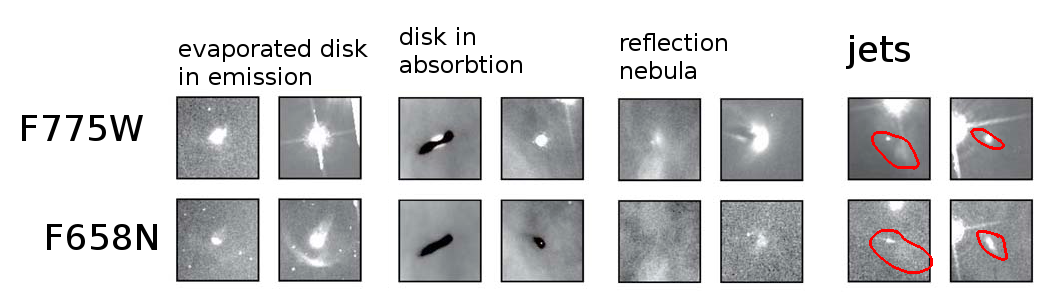
\includegraphics[width=\textwidth]{ONCACS.png}
    \caption{Examples of different objects detected in an ACS survey of the Orion Nebula Cloud by \citet{2008AJ....136.2136R}, each column shows one object in two different filters (\emph{top}: F775W is SDSS $i'$, \emph{bottom}: F658N covers the H$\alpha$ line). For each category, two objects are shown. Note how some features stand out in the emission line, while others are visible in the broad-band.}
    \label{fig:ONCACS}
\end{figure}

\subsection{Jet sources and jet launching}
It is unknown how jets are launched and collimated, but ultimately, they have
to be powered by the gravitational energy released in the accretion process. In
close-by stars, jets are layered like an onion where slower, outer layers are
surrounded by denser and faster layers inside \citep{2000ApJ...537L..49B}. The
innermost layers can reach a few 1000~km/s for jets from massive stars and heat
up to X-ray emitting temperatures, but the bulk of the mass is neutral or
moderately ionized and emits H$\alpha$, or optical emission lines such as
[O~{\sc i}] 6300\AA{} or [O~{\sc iii}] 5007\AA{} (Fig.~\ref{fig:reiter},
left or Fig.~\ref{fig:ONCACS}, rightmost sources). The sample of well-studied jets is surprisingly small, especially for
later stages of star formation and lower mass sources where jets are less
powerful and thus fainter and harder to find; such micro-jets are sometimes
only a few arcseconds long, with the brightest part of the emission close to
the star. From the ground, those jets can only be seen with adaptive optics
imaging and will not be found in large-scale surveys; but they are easily
visible in HST images. Even for more powerful jets, which are resolved at
resolutions typical for ground-based seeing, we often require high-resolution
imaging to identify the jet source.


\subsection{Knots in jets}
Jets are not homogenous structures, but contain knots. These can be due to mass-ejection events in the past, and, since mass ejection and accretion are related, contain a fossil archive of previous accretion rates \citep{2014A&A...563A..87E}. However, as knots move away from the source, they become fainter. If jet emission switches on an off in a source, there may be no indication of a jet seen in the star today; thus surveys looking for jets would not target those sources, however, fossil records of previous jet event may still be out there in the form of faint emission regions, at some distance form the source. HST imaging in a blind search in H$\alpha$ and [O~{\sc i}] is a promising way to find those features, if the exisit. This is actually easier in low-mass star forming regions where the source density if lower and thus the likely jet source can be identified, even if emission is not seen close to it.

\subsection{Disk evolution and evaporation}

Understanding external photoevaporation is also important for the history of the solar systems and the formation of our Earth \citep{2015ApJ...815..112K}.

Theoretically, we expect that the livetimes of disks depend strongly on the formation environment, where massive stars in dense clusters should evaporated disks within a Myrs or so and close encounters can strip additional material from the disks \citep[e.g.][]{2004ApJ...611..360A,2019MNRAS.485.1489W,2019arXiv190211094N}but there are recent indications that external photo-evaporation can be important even in low-mass star forming regions \citep{2017MNRAS.468L.108H}.
There are two ways to study this observationally: Look how disk properties in a massive cluster change with distance from the most massive members \citep{2018ApJ...860...77E}, or compare clusters of different mass. Our proposed study can help with both, giving us high-resolution observations of low-mass star forming regions where normally one would not invest much time on a blind survey to find disks in imaging, and images of massive clusters, a little further away from the objects usually studied.




\subsection{Multiplicity}
A large fraction of all young stars forms in binaries or higher order multiples, yet many questions about the evolution of multiple systems remain unsolved. First, simply knowing the fraction of multiple systems and the mass and radius distribution of companions can tell us under what conditions companions grow in the envelops of disk of the primary (like planets) versus how the envelope forms two stars. If we can image disks or outflows of at least one of the stars, we can also start to probe if orbital plane and individual disks are aligned.

For close-in binaries, the companion will obviously change the evolution of the primary's disk, e.g. by triggering episodic accretion \citep{2013ApJ...766...62G}, and thus possibly reducing the time and the mass reservoir available for planet formation. For binaries with separations comparable to the size of a disk in the T Tauri phase (a few hundred au) this is less clear. In the well-studied case of RW~Aur~A and B a tidal stream connects the disks \citep{2006A&A...452..897C}. However, to study these effects in a sample, we first need an accurate census of multiplicity and how this might change with the mass of the central star and its formation environment.

For all these reasons, we need to identify more systems with companions. One of
the best methods to do that is imaging from space in $R$ or $I$ or the near-IR where the contrast between the primary and a lower mass secondary is less extreme than in, e.g.\ the $V$ band. 

\citet{2001A&A...379..147D} find about 20\% of their sample in the young
cluster NGC 6611 have a companion in the range 200-3000~au, where the companion
has at least a tenth of the mass of the primary. With HST's sub-arcsecond PSF,
we can detect a K8 companion at 200~au distance from a moderately bright
primary for star forming regions at 1 kpc, and we can perform reliable photometry on companions separated by 500~au or so. 


\section{Estimating the yield of the proposed survey}
Our proposed observing strategy is very similar to the atlas of protoplanetary disks in the Orion Nebula by \citet{2008AJ....136.2136R}. Their survey covers about 450~arcmin$^2$ in $B$, $V$, H$\alpha$, $I$, and $z$ with average exposure times about 400~s. They detect about 3200 compact sources and 219 sources with circumstellar matter. The largest fraction of those (178) are externally ionized disk in emission; 36 disks are seen in extinction against the bright nebula in the background. Five objects show jets without an apparent disk (meaning that the disk is likely to be smaller because the objects are more evolved). Figure~\ref{fig:ONCACS} shows examples of these detections. 

In a request for 100 pure-parallel obits we will sample about 0.3 sq deg of
area in several star forming clouds, likely including both close-by low-mass
star forming regions and higher-mass star forming regions at a larger distance.
%This is several orders of magnitude less than the large \emph{Spitzer} surveys
%of star forming regions, but it will still be the largest dataset available
%with the superb spatial resolution that HST offers and the number of filters we
%plan to use.
 Ground-based based surveys are typically only done in broad-band
filters \citep[IPHAS, which also includes an H$\alpha$ filter is an
  exception]{2005MNRAS.362..753D} and without adaptive optics, thus the
space-based \emph{HST} images that we will obtain will be superior in spatial
resolution, depth, and coverage of spectral features. For the primary
\emph{HST} observations, observers often choose ``special'' locations,
e.g.\ the brightest and most active stars in a star forming region. A census
measuring the effect of photoevaporation in these regions does not necessarily
represent the typical state of star formation; in fact, any concentration of
observations in the center of a star forming region (where the highest number
of sources is found) biases a study towards effects of dense
environments. While our points will not be truly randomly distributed, they
will cover a range of star forming environments in different clusters that has
not been studied with such high spatial resolution and such uniform filter
coverage before.

Depending on the star forming region where the primary targets are located, the
number of objects we can detect will differ. If the primary targets are in
dense star forming regions such as the Orion Nebula Cloud or Carina, we are
virtually guaranteed to see several young stars, cloud structures, disks and
outflows for any target location; on the other hand, if the primary targets are
in close-by low-density star forming regions such as Taurus, we may find some
field to devoid of cluster members. 


Pure-parallel surveys have taken deep images in star forming regions before and
have been used for extragalactic astronomy \citep{2007A&A...468..823S} but also
to search for ultracool objects such as L and T dwarfs in the galaxy
\citep{2005ApJ...631L.159R}. These studies show the potential for serendipitous
science from deep high-resolution imaging beyond the science justification we
lay out here. We analyzed some of this data and verified that structures of the
molecular cloud are indeed visible in great detail; however, all those data are
taken in wide filters only while we propose additional observations in narrow
band filter which probe particular conditions in irradiated clouds, disks and
jets.


%%%%%%%%%%%%%%%%%%%%%%%%%%%%%%%%%%%%%%%%%%%%%%%%%%%%%%%%%%%%%%%%%%%%%%%%%%%

%   2. DESCRIPTION OF THE OBSERVATIONS
%       (See https://hst-docs.stsci.edu/display/HSP/HST+Cycle+27+Preparation+of+the+PDF+Attachment)
%
%
\describeobservations   % Do not delete this command.
% Enter your observing description here.
We are requesting observations in pure parallel mode, meaning that our images will be taken when some other program uses COS or STIS are prime instruments and happens to look at a star forming region. Thanks to the ULLYSES program, we know that a few dozen orbits of spectroscopic data will be taken in star forming regions, in addition to any GO programs for spectroscopy of young stars that may be approved in this cycle by the TAC. In Phase II, STScI will generate a list of such primary orbits, which may be suitable for the execution of the observations we propose for here, but as a pure-parallel program, we have no influence over the setup of those observations. That means that the exact pointing, orientation and number of dither positions will be determined by the primary science program. Thus, we describe a general set-up of the observations here, but details will have to be adjusted in Phase II.

To reach our science objectives, we request to obtain images in two broadband (SDSS $r'$ and $i'$) and two narrow-band filters (H$\alpha$ and an oxygen line). In high-mass star forming regions, [O~{\sc iii}] isa good tracer of hot nebular gas, but in low-mass star forming regions, [O~{\sc iii}] 5007\AA{} is weak or absent. The WFC3 has an [O~{\sc i}] 6300\AA{} filter, while the ACS/WFC does not and we propose to use the [O~{\sc i}] 6300\AA{} filter with the WFC3 for targets in low-mass star forming regions. Table~\ref{tab:setup} summarizes the filters to be used.
For a typical usable orbit time of about 2800~s after acquisition, we can take one exposure of 540~s in each filter. Once we know the exact duration of the orbit (which depends on the position and roll angle specified by the primary target), we will optimize the exposure times to reduce the time lost to buffer dumps and filter changes.

If we have only one orbit with a specific pointing, we will perform imaging with the WFC3 because it is located closer to the STIS or COS FOV. In a star forming region, a STIS or COS observation is most likely centered on a bright, active star and thus observing closer to it increases the chances to find irradiated cloud or outflow features. 

\begin{table}[htbp]
    \centering
    \begin{tabular}{c|ccc}
    \hline\hline
           & WFC3 & WFC3 & ACS/WFC \\
        star forming region & high-mass & low-mass & any\\
        \hline
        SDSS $r'$ & F625W & F625W & F625W \\
        SDSS $i'$ & F775W & F775W & F775W\\
        H$\alpha$ & F656N & F656N & F658N\\{}
        [O~{\sc iii}] 5007\AA{} & F502N & -- & F502N\\{}
        [O~{\sc i}] 6300\AA{}& -- & F631N & -- \\
        \hline
    \end{tabular}
    \caption{Filters to be used for observations in high and low-mass star forming regions.}
    \label{tab:setup}
\end{table}


Commonly, spectroscopic observations last for more than one orbit and thus it is likely that we will have access to more than one parallel orbit with almost the same pointing. In this case, we will use the second orbit for observations with ACS/WFC (see table~\ref{tab:setup}). ACS has a FOV a few arcmin away from WFC3. Should more than two orbits be available with the same pointing, we will repeat the WFC3 and ACS observations to detect fainter features and to take advantage of multiple dither positions (if the primary observation dithers) and to obtain more exposures in each filter to help with cosmic ray rejection. 

We looked at STIS and COS observations in star forming regions as well as previous pure-parallel programs in the archive and find that it is not uncommon to have 5-10 orbits with very similar pointings; which would give us a summed exposure time of about one orbit per filter. For longer observations, HST will often observe the primary target at different roll angles and thus WFC3 and ACS will see a different area on the sky even if the primary program observes the same target for a large number of orbits. Adding up the FOV for WFC and ACS, we think that with a request of 100 pure parallel orbits we will sample 300-400 sq arcmin deg of star forming region (assuming on average 3-5 orbits with the same pointing) - not a large area, but since this is a pure parallel program it does not cost any primary orbits to perform such a survey.

Just to give some examples for our sensitivity: In a single orbit (exposure 540~s in each filter), we can detect an M7 star in a close star forming region (130~pc) or an M2 at 0.5~kpc; sources like this should also be part of 2MASS, giving us fluxes in five colors so that we can fit the spectral type, extinction, and check for the presence of a disk in the spectral energy distribution (SED) \citep{2007ApJS..169..328R}.
See the figures in the text above for examples of resolved cloud or jet emission features that were found in observations comparable to what we propose here.

Note that this is a request for a blind survey. Since the targets of the primary observations are not known, we do not know what number of features we will find. Obviously, more observing times will allow us to cover a larger area or go deeper (depending on the distribution of targets for the primary observations). At the same time, this program is still useful if only a smaller number than the requested 100 orbits is granted or available; in this case we will simply survey a smaller area (or not as deep, depending on the distribution of primary targets).



%%%%%%%%%%%%%%%%%%%%%%%%%%%%%%%%%%%%%%%%%%%%%%%%%%%%%%%%%%%%%%%%%%%%%%%%%%%

%   3. SPECIAL REQUIREMENTS
%       (See https://hst-docs.stsci.edu/display/HSP/HST+Cycle+27+Preparation+of+the+PDF+Attachment)
%
%
\specialreq             % Do not delete this command.
% Justify your special requirements here, if any.
None.

%%%%%%%%%%%%%%%%%%%%%%%%%%%%%%%%%%%%%%%%%%%%%%%%%%%%%%%%%%%%%%%%%%%%%%%%%%%

%   4. COORDINATED OBSERVATIONS
%       ((See https://hst-docs.stsci.edu/display/HSP/HST+Cycle+27+Preparation+of+the+PDF+Attachment)
%
%
\coordinatedobs          % Do not delete this command.
% Enter your coordinated observing plans here, if any.
None.

%%%%%%%%%%%%%%%%%%%%%%%%%%%%%%%%%%%%%%%%%%%%%%%%%%%%%%%%%%%%%%%%%%%%%%%%%%%

%   5. JUSTIFY DUPLICATIONS
%       (See https://hst-docs.stsci.edu/display/HSP/HST+Cycle+27+Preparation+of+the+PDF+Attachment)
%
%
\duplications           % Do not delete this command.
% Enter your duplication justifications here, if any.
If a region on the sky that would we available to this program has been observe before with these or similar filters, the new observations still add additional data to look for fainter objects, or, for brighter objects, to study their proper motion (e.g\ the expansion of a gas bubble or the motion of a know in a jet).

%%%%%%%%%%%%%%%%%%%%%%%%%%%%%%%%%%%%%%%%%%%%%%%%%%%%%%%%%%%%%%%%%%%%%%%%%%%
\bibliographystyle{aa} % style aa.bst
\bibliography{biblio}


\end{document}          % End of proposal. Do not delete this line.
                        % Everything after this command is ignored.
